\documentclass{letter}
\usepackage[margin=0.75in]{geometry}
\usepackage{amsmath}
\usepackage{amssymb}
\usepackage{enumerate}
\usepackage{tikz}
\usepackage{pgfplots}
\pgfplotsset{compat=1.8}

\pgfplotsset{vasymptote/.style={
		before end axis/.append code={
			\draw[densely dashed] ({rel axis cs:0,0} -| {axis cs:#1,0})
			-- ({rel axis cs:0,1} -| {axis cs:#1,0});
		}
	}}

\begin{document}
	\begin{center}
		\LARGE Math137 - November 9'th, 2015\\
		\large Intro to Curve Sketching
	\end{center}
	\vspace{0.25 in}
	\underline{\textbf{Curve Sketching - General Procedure}}
	
	All necessary information for sketching $y=f(x)$ can be obtained from the following:
	
	\begin{enumerate}[1)]
		\item $f(x)$
		\begin{itemize}
			\item[-] Determine domain of the function.
			\item[-] $x, y$ Intercepts
			\item[-] Asymptotes
		\end{itemize}
		\item $f'(x)$
		\begin{itemize}
			\item[-] Determine intervals of increase and decrease by applying the Increasing/Decreasing Function Test (listed below).
			\item[-] Determine local minimums and maximums by applying the First Derivative Test (listed below).
		\end{itemize}
		\item $f''(x)$
		\begin{itemize}
			\item[-] Determine Concavity of $f$ by applying the Concavity Test (listed below)
			\item[-] Determine POI's (Points of Inflection).
		\end{itemize}
	\end{enumerate}
	
	\underline{\textbf{Increasing/Decreasing Function Test}}
	\begin{enumerate}[a)]
		\item If $f'(x) > 0$ on some interval $I$, then $f(x)$ is increasing on the interval $I$.
		\item If $f'(x) < 0$ on some interval $I$, then $f(x)$ is decreasing in the interval $I$.
	\end{enumerate}
	\underline{\textbf{First Derivative Test}}
	
	Suppose $c$ is a critical point of a continuous function $f$.
	\begin{enumerate}[a)]
		\item If $f'$ changes from positive to negative at $c$, then $f$ has a local maximum at $c$.
		\item If $f'$ changes from negative to positive at $c$, then $f$ has a local minimum at $c$.
		\item If $f'$ does not change sign at $c$, then there is no local maximum or minimum at $c$.
	\end{enumerate}
	\underline{\textbf{Concavity Test}}
	\begin{enumerate}[a)]
		\item If $f''(x) > 0$ for all $x \in$ an interval $I$, then $f(x)$ is concave up on $I$.
		\item If $f''(x) <0$ for all $x \in$ an interval $I$, then $f(x)$ is concave down on $I$.
	\end{enumerate}
	\underline{\textbf{Inflection Points}}
	
	Inflection points occur where $f''(x)$ changes sign and $f$ is continuous. If $f''(c) = 0$, $c$ is a \textbf{possible} inflection point. We still must check that the sign is different on the left and right side of $c$ to confirm.
	\pagebreak\\
	\underline{\textbf{Example Sketch}}
	
	Sketch the following function: $y = f(x) = \frac{x^3}{(1+x)}$
	\begin{enumerate}[i)]
		\item Lets begin by finding out zero's (x intercepts):
		\begin{flalign*}
			x^3 &= 0&\\
			x &= 0
		\end{flalign*}
		\item Now the y intercept:
		\begin{flalign*}
			y &= \frac{0^3}{(1+0)}&\\
			&= 0
		\end{flalign*}
		\item Vertical Asymptotes:
		\begin{flalign*}
			(1+x) &= 0&\\
			x &= -1
		\end{flalign*}
		For asymptote behavior, we'll plug in a number very close to the asymptote on either side and see if we have a positive or negative number. We're only concerned with positive-ness and negative-ness (The actual value is irrelevant to us) so I'll represent these numbers by + signs or - signs\\
		
		First, lets try just to the left of our asymptote, $x = -1.01$
		\begin{flalign*}
			f(x) &= \frac{(-1.01)^3}{(1 + (-1.01))}&\\
			&= \frac{-}{-}\\
			&= +
		\end{flalign*}
		So as $x$ approaches -1 from the left, $y$ tends to $\infty$. Now we'll try the other side.
		\begin{flalign*}
			f(x) &= \frac{(-0.99)^3}{(1 + (-0.99))}&\\
			&= \frac{-}{+}\\
			&= -
		\end{flalign*}
		As $x$ approaches -1 from the right side, $y$ tends to $-\infty$.
		\item Critical Points:
		\begin{flalign*}
			f(x) &= \frac{x^3}{1+x}&\\
			f'(x) &= \frac{(3x^2)(1+x)+(x^3)(1)}{(1+x)^2}\\
			&= \frac{x^2(3+2x)}{(1+x)^2}
		\end{flalign*}
		$\therefore$ Critical values at $x=0, -1, \frac{-3}{2}$\\
		
		Now we'll check positiveness/negativeness of our derivative to find increasing/decreasing intervals of our original function.\\
		
		\begin{tabular}{c|c|c|c|c}
			& $x<\frac{-3}{2}$ & $\frac{-3}{2} < x < -1$ & $-1 < x < 0$ & $x > 0$\\
			\hline
			$x^2(3+2x)$& - & + & + & + \\
			$(1+x)^2$& + & + & + & + \\
			$f'$& - & + & + & +\\
			$f$& dec. & inc. & inc. & inc.
		\end{tabular}\\
		\pagebreak\\
		From this, we can see the intervals on which our function is increasing and decreasing. We can also find local maxima and minima anywhere where our derivative changes sign \textbf{and} the function exists.\\
		We see we have one derivative sign change at $x=\frac{-3}{2}$. Our original function $f$ is continuous so long as $x \not= -1$, so the value is included in our function. Therefore, we can conclude $x=\frac{-3}{2}$ is a local minimum. We'll want the $y$ value as well, so let's calculate that.
		\begin{flalign*}
			f(\frac{-3}{2}) &= \frac{(\frac{-3}{2})^3}{1+\frac{-3}{2}}&\\
			&= (\frac{-27}{8})(\frac{2}{-1})\\
			&= \frac{27}{4}
		\end{flalign*}
		$\therefore$ We have a minimum at $(-1.5, 6.75)$.
		\item Now we'll do concavity and points of inflection.
		\begin{flalign*}
			f'(x) &= \frac{(x^2)(3+2x)}{(1+x)^2}&\\
			f''(x) &= \frac{[(2x)(3+2x)+(x^2)(2)] - [(x^2)(3+2x)(2)(1+x)]}{(1+x)^4}\\
			&= \frac{(6x + 4x^2 + 2x^2)(1 + 2x + x^2) - (3x^2 + 2x^3)(2 + 2x)}{(1+x)^4}\\
			&= \frac{6x + 12x^2 + 6x^3 + 4x^2 + 8x^3 + 4x^4 + 2x^2 + 4x^3 + 2x^4 - 6x^2 - 6x^3 - 4x^3 - 4x^4}{(1+x)^4}\\
			&= \frac{2x^4 + 8x^3 + 12x^2 + 6x}{(1+x)^4}\\
			&= \frac{2x(x^3 + 4x^2 + 6x + 3)}{(1+x)^4}\\
			&= \frac{(2x)(x+1)(x^2+3x+3)}{(1+x)^4}\\
			&= \frac{(2x)(x^2+3x+3)}{(1+x)^3}
		\end{flalign*}
		Lovely. The critical values of our second derivative are: $x = 0, -1$. Now we do the same thing as we did with the first derivative: Find where this function is increasing and decreasing using the critical values as interval endpoints.\\
		
		\begin{tabular}{c|c|c|c}
			& $x<-1$ & $-1 < x < 0$ & $x > 0$\\
			\hline
			$(2x)(x^2 + 3x + 3)$ & - & - & +\\
			$(1+x)^3$ & - & + & +\\
			$f''(x)$ & + & - & +\\
			$f(x)$ & conc. up & conc. down & conc. up
		\end{tabular}\\
		
		We have possible points of inflection at $x= -1, 0$.\\
		The function does not exist at $x = -1$, so it cannot be a point of inflection.\\
		The function exists and is continuous at $x = 0$, so $x = 0$ is a POI.
	\end{enumerate}
	Now, lets recap all we've learned about our function.\\
	
	\begin{minipage}[t]{0.33\textwidth}
		$x$ intercepts: $x=0$\\
		$y$ intercept: $y=0$\\
		V asymptote: $x=-1$\\
		Behavior:\\
		From the left, y approaches $\infty$\\
		From the right, y approaches $-\infty$
	\end{minipage}
	\begin{minipage}[t]{0.33\textwidth}
		Increasing:\\
		$x \in (-\infty, \frac{-3}{2}) \cup (-, \infty)$\\
		Decreasing:\\
		$x \in (\frac{-3}{2}, -1) \cup (-1, 0)$\\
		Local min at $(-1.5, 6.75)$
	\end{minipage}
	\begin{minipage}[t]{0.33\textwidth}
		Concave Up:\\
		$x \in (-\infty, -1) \cup (0, \infty)$\\
		Concave Down:\\
		$x \in (-1, 0)$\\
		POI at $x=0$
	\end{minipage}\\
	\pagebreak\\
	That's a lot of information. Wow. Now we can create a very accurate graph of this function. 
	
	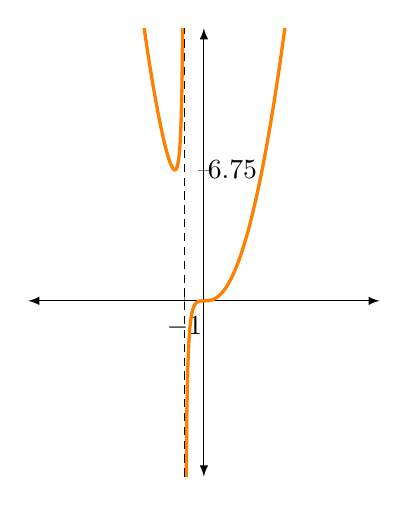
\begin{tikzpicture}
	\begin{axis}[
	axis equal image,
	axis lines=middle,
	xmin=-5,xmax=5,
	ymin=-5,ymax=10,
	enlargelimits={abs=1cm},
	axis line style={latex-latex},
	yticklabel style={anchor=west},
	ytick={6.75},
	xtick={-1},
	vasymptote=-1,
	]
	% This doesn't clip to y=-10:10 nicely
	% because there are too few samples near the asymptote:
	\addplot[very thick, orange, domain=-5:5,samples=200, restrict y to domain=-20:115]
	{(x^3)/(1+x)};
	
	
	\end{axis}
	\end{tikzpicture}\\
	This is what our graph should look like. Don't mind the asymptote x marker, this was my first graph in latex, I'll figure out how to fine tune the graphs eventually!
\end{document}